
        \documentclass{article}
        \usepackage{tikz}
        \begin{document}
            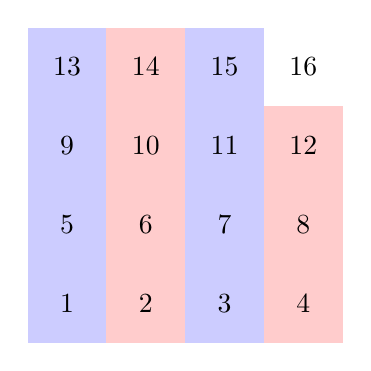
\begin{tikzpicture}[thick]  
    \node[fill=blue!20, minimum size=1cm, inner sep=0pt] at (0,0) {$1$};
\node[fill=red!20, minimum size=1cm, inner sep=0pt] at (1,0) {$2$};
\node[fill=blue!20, minimum size=1cm, inner sep=0pt] at (2,0) {$3$};
\node[fill=red!20, minimum size=1cm, inner sep=0pt] at (3,0) {$4$};
\node[fill=blue!20, minimum size=1cm, inner sep=0pt] at (0,1) {$5$};
\node[fill=red!20, minimum size=1cm, inner sep=0pt] at (1,1) {$6$};
\node[fill=blue!20, minimum size=1cm, inner sep=0pt] at (2,1) {$7$};
\node[fill=red!20, minimum size=1cm, inner sep=0pt] at (3,1) {$8$};
\node[fill=blue!20, minimum size=1cm, inner sep=0pt] at (0,2) {$9$};
\node[fill=red!20, minimum size=1cm, inner sep=0pt] at (1,2) {$10$};
\node[fill=blue!20, minimum size=1cm, inner sep=0pt] at (2,2) {$11$};
\node[fill=red!20, minimum size=1cm, inner sep=0pt] at (3,2) {$12$};
\node[fill=blue!20, minimum size=1cm, inner sep=0pt] at (0,3) {$13$};
\node[fill=red!20, minimum size=1cm, inner sep=0pt] at (1,3) {$14$};
\node[fill=blue!20, minimum size=1cm, inner sep=0pt] at (2,3) {$15$};
\node[fill=white!20, minimum size=1cm, inner sep=0pt] at (3,3) {$16$};

            \end{tikzpicture}
        \end{document}
    